\documentclass[a4paper,12pt]{article}

\usepackage[utf8]{inputenc}
\usepackage{graphicx}
\usepackage{amsmath}
\usepackage[margin=1in]{geometry}
\usepackage{caption}
\usepackage{lmodern}
\usepackage{parskip}
\usepackage{textcomp}
\usepackage{fancyhdr}

\pagestyle{fancy}
\fancyhf{}
\rhead{Feasibility Analysis -- GD\&T Drawing AI}
\lhead{Problem Statement}
\rfoot{\thepage}

\title{\textbf{Problem Statement -- Automating Drawing Analysis for Tolerance Feasibility}}
\author{Your Name \\ PSM Protech GmbH Project}
\date{\today}

\begin{document}

\maketitle

\section*{Customer Problem (Engineering Perspective)}

In the quotation phase at PSM Protech GmbH, customers submit detailed mechanical drawings containing dimensions, tolerances, GD\&T symbols, and various callouts (commonly enclosed in ovals). Engineers must manually extract and interpret these symbols and values to assess manufacturability and process feasibility.

This manual extraction process is slow, error-prone, and highly repetitive --- especially since a single drawing can contain over 500 callouts and multiple versions. Missing critical tolerances such as $\pm 0.01~\text{mm}$ can lead to incorrect quotations, increased production costs, or delays. Automating this analysis can significantly improve speed, accuracy, and consistency in early design evaluation.

\section*{Technical Problem (Machine Learning/Computer Vision Perspective)}

To automate the interpretation of these engineering drawings, we propose a multi-stage pipeline using AI and computer vision:

\begin{itemize}
  \item \textbf{Object Detection (YOLOv8):} Detect oval callouts and GD\&T frames (feature control frames) in the drawing.
  \item \textbf{Image Classification:} Classify detected geometric tolerance symbols (e.g., flatness, roundness, perpendicularity) according to ISO 1101.
  \item \textbf{Optical Character Recognition (OCR):} Extract numerical tolerance values (e.g., $\pm 0.05$, \text{O}10.2), text annotations (e.g., ``CC'', ``3x''), and datums (A, B, C).
  \item \textbf{Rule-Based Classification:} Use customer-defined feasibility rules to classify dimensions as either feasible (green) or critical/infeasible (red).
  \item \textbf{(Optional) Version Comparison:} Highlight changes between drawing revisions for re-review.
\end{itemize}

\begin{figure}[h!]
  \centering
  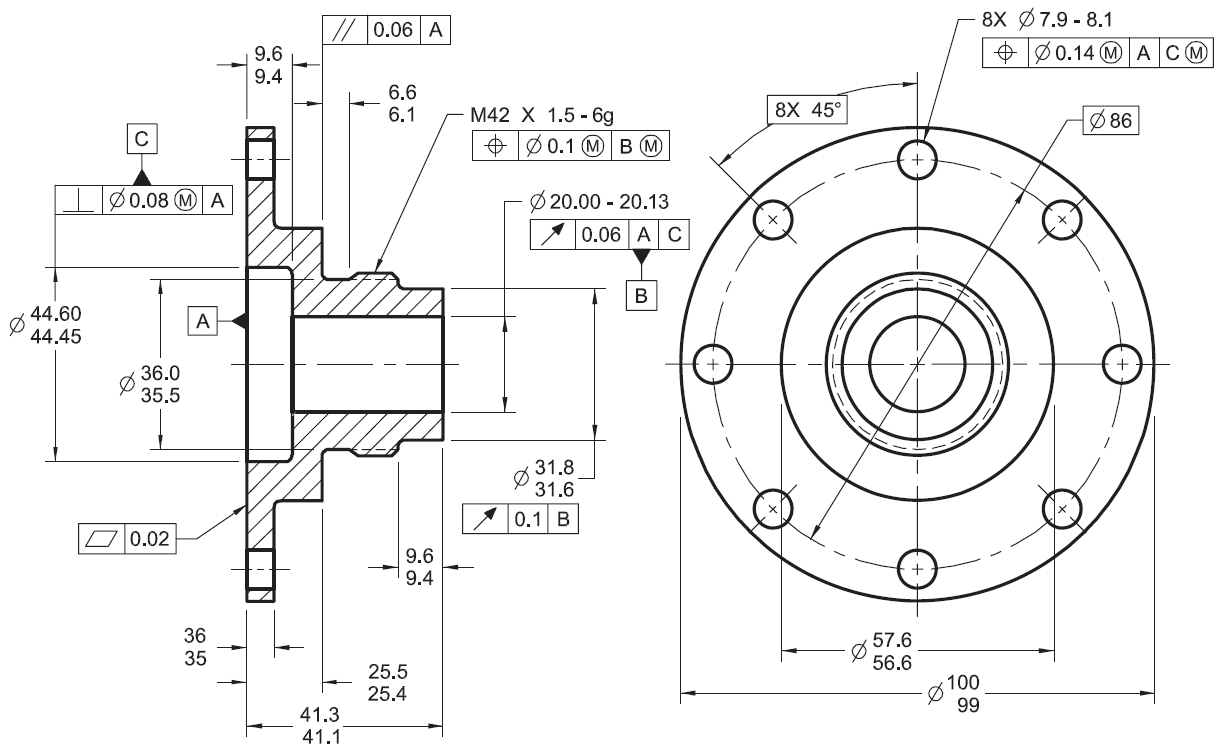
\includegraphics[width=0.9\textwidth]{images/GDD-Drawing_Problemstatement.png} % Make sure this path is correct
  \caption{AI-based detection pipeline: YOLO identifies oval callouts and symbol blocks; image classification labels GD\&T symbols; OCR extracts values for feasibility checking.}
  \label{fig:pipeline_example}
\end{figure}

\end{document}